%%!TEX root = dissertation.tex

\chapter{Croslinguistic uniformity for VOT}

\label{Uniformity}

\section{Introduction}
A consequence of bilingualism is that individuals must navigate overlapping segment inventories \citep{flege_2021_slmr}. This paper is concerned with the question of what languages share, if anything, in the representation of speech sounds. Most prior work has focused on sounds that are phonologically similar, yet phonetically distinct, as with the comparison between initial voiceless stops in English (long-lag) and Spanish (short-lag). Despite the substantial phonetic differences, these sounds are clearly linked in the bilingual mind \citep{fricke_2016_phonetic,antoniou_2010_context,goldrick_2014_switching,sundara_2006_production}. The studies cited here all examine initial voice-onset time (VOT) for bilinguals who speak English and a language with a different initial voicing contrast---Greek, Spanish, or French---and demonstrate convergence in two ways. First, VOT is shorter for English initial stops produced by bilinguals, when compared to monolingual control groups. This result is attributed to influence on English long-lag stops from the short-lag category in the other language. Second, bilinguals appear more likely to produce lead voicing in initial English voiced stops compared to English monolinguals \citep{sundara_2006_production}. In both cases, evidence of crosslinguistic influence arises from comparing bilinguals to monolinguals. Corpus research demonstrates that Spanish-English bilinguals produce shorter, more Spanish-like VOT in the lead up to an English-to-Spanish code switch \citep{fricke_2016_phonetic,bullock_2009_sociophonetics}. The studies mentioned so far focus on VOT, but represent a small subset of the crosslinguistic influence literature. There are many examples of contrasts that are maintained across languages, yet still subject to crosslinguistic influence---for example, with vowels \citep{guion_2003_systems}, laterals \citep{amengual_2018_laterals,barlow_2014_aoa}, and fricatives \citep{peng_1993_influence}). 

The ability to examine crosslinguistic influence between similar sounds hinges on the presence of an observable difference, at least under some set of conditions. The sounds typically selected are not discussed as being the same---phonetic character choice notwithstanding. As such, links tend to be described as connecting similar and subject-to-influence sounds that ultimately have distinct representations \citep{antoniou_2010_context,simonet_2016_bilingualism,bullock_2009_sociophonetics}. In the revised Speech Learning Model (SLM-r) \citep{flege_2021_slmr}, these examples would be considered composite categories---combined distributions of phonetic information from linked categories that presumably retain ``peaks'' for each language. While composite categories are widely attested, there are fewer good examples of full category convergence, at least in the early bilingualism literature. One example comes from a lab-based study of Mandarin-English bilingual children in which highly proficient 5--6 year olds did not differ in VOT across Mandarin and English long-lag stops, despite differences across the monolingual comparison groups \citep{yang_2019_vot}. This suggests that the difference is either too small to maintain or that 5--6 year old children have not yet mastered it. The claims in \citep{yang_2019_vot} should be tempered, however, as language mode was not well-controlled for and adult bilingual behavior was not considered.

Despite some inroads, there is nonetheless a distinct paucity of work examining highly similar speech sounds across languages, even when such a comparison would make sense. A recent study of crosslinguistic influence in Cantonese-English bilinguals compares English long-lag and Cantonese short-lag stops in the context of a language switching paradigm \citep{tsui_2019_switching}. While this comparison clearly reflects the need for stimuli to be acoustically distinct beforehand, it glosses over the fact that both languages contrast short-lag and long-lag VOT in initial position. The best candidates for linkages---and accompanying crosslinguistic influence---should be the long-lag stops in each language. The null result with balanced bilinguals is thus unsurprising. This is not to suggest that the \citep{tsui_2019_switching} would have gotten more insightful results by comparing long-lag to long-lag, but rather to highlight that paradigms designed to modulate crosslinguistic influence tend to focus on \textit{telling things apart}, as opposed to \textit{telling things together}.

The idea of telling things apart or together fits within the SLM-r framework \citep{flege_2021_slmr}, where categories from different languages exist in a shared phonetic space and are subject to constraints from the perceptual an productive systems: don't get too close to each other in perception, and don't get too complicated in production \citep{guion_2003_systems,lindblom_1988_universals, flege_1995_slm}. This framework assumes that close proximity leads to instability, but fails to define what counts as close. Considering the proximity that bilinguals are capable of maintaining, this is not a trivial point to make. Assuming that convergence is an outcome of proximity at least sometimes, the original SLM would argue that if two segments sound like the same duck, then they must in fact be the same duck (i.e., share an underlying representation). Note, however, that this conclusion does not necessarily apply to composite categories where differences persist despite crosslinguistic influence.
 
English and Cantonese initial long-lag stops are strong candidates for shared underlying representation, because they exhibit both phonetic and phonological \textit{similarity} akin to the difference for Mandarin and English in \citep{yang_2019_vot}. In an overview chapter on crosslinguistic segment similarity, \citep{chang_2015_similarity} argues that the notion of similarity is best captured abstractly, by relative within-inventory position as opposed to physical characteristics. In an example from \citep{chang_2015_similarity}, English and Mandarin /\textipa{u}/ are considered to be linked---both occupy the highest, backest, rounded position---despite English /\textipa{u}/-fronting rendering it more physically similar to Mandarin /\textipa{y}/. This abstract ``relative phonetics'' elegantly accounts for various phenomena \citep{chang_2015_similarity}, while simultaneously shying away from making claims about whether or not segments share representation or theoretical phonological specifications across languages. 

To summarize, most work in crosslinguistic influence has focused on phonologically-similar yet phonetically-distinct pairs of segments, which are not strong candidates for shared representation. This common focus on telling things apart is likely an artifact of commonly-used paradigms requiring differences to detect influence. Alternatively, comparisons of categories that already show strong evidence of similarity may be taken for granted and not considered an interesting problem to focus on, despite the nature of representation being a key focus of psycholinguistics in general---especially in perception \citep{samuel_2020_resist}. In the interest of understanding representation, the best candidates would be the hardest to distinguish in the first place. 

The present study is focused instead on \textit{telling things together}, and in doing so extends the articulatory uniformity framework to the study of multilingual segment inventories. Articulatory uniformity is conceptualized as a constraint on within-talker phonetic variation, in which phonological primitives (e.g., features) are implemented systematically in speech production \citep{chodroff_2017_structure,faytak_2018_uniformity,menard_2008_invariance}. Put differently, if a set of segments share a phonological feature, that feature should be implemented with the same phonetic target or articulatory gesture (which may or may not have an acoustic consequence). This systematicity has been observed for in vowel height \citep{menard_2008_invariance}, tongue shape \citep{faytak_2018_uniformity}, fricative peak frequency, and stop consonant VOT \citep{chodroff_2017_structure}. In the case of VOT, the relationship between laryngeal gesture and acoustic consequence is clear. While there are straightforward ties to theoretical phonology from articulatory uniformity, the selection of a particular framework is not a straightforward task in a bilingual context. English and Cantonese stops are typically analyzed with different distinctive features---[voice] and [spread glottis], respectively---despite surfacing with long-lag VOT in initial position and occupying the same relative position. The study reported here focuses only on the relative phonetics and sidesteps theoretical phonology for the time being. This is consistent with the argument that theoretical linguistic descriptions do not always neatly map onto psycholinguistic phenomena \citep{samuel_2020_resist}.

Within-language uniformity has been observed for initial stops in non-native English, such that the relationship between stops for an individual is clear even if between-talker variability is larger than for native speakers \citep{chodroff_2019_l2}. However, the uniformity framework has not yet been extended to early bilingual speech, in particular as a mechanism for comparing how bilinguals produce similar sounds in each of their languages. Extending the framework in this way, however, follows the conceptualization of uniformity arising from articulatory reuse \citep{faytak_2018_uniformity}. In the case of an early Cantonese-English bilinguals, consider the initial stop [k\textsuperscript{h}] with a mean VOT of 80 ms in American English \citep{lisker_1964_vot} and 91 ms in Hong Kong Cantonese \citep{clumeck_1981_cantonese}. While these values are objectively different---though based on small sample sizes---it seems that using the same laryngeal timing gesture in this case would be advantageous given the small difference across monolingual populations, that may or may not be perceptible. While this remains an empirical question, it follows the finding that bilingual Mandarin-English children did not distinguish between languages in VOT \citep{yang_2019_vot}. Following the predictions of the SLM-r \citep{flege_2021_slmr}, this work suggests that long-lag items of minimally distinct VOT would assimilate or dissimilate, but not be stable in such close proximity. Thus, the present study asks: Do Cantonese-English bilinguals uniformly produce long-lag stops within and across each of their languages? Leveraging the methodology from \citep{chodroff_2017_structure,chodroff_2018_predictability,chodroff_2019_l2} allows for a new perspective on the structure of variation and nature of representation in bilinguals, and facilitates the study of already similar speech sounds, in ways that other paradigms do not. As may be clear from the framing of the introduction, the hypothesis was that bilinguals would indeed exhibit crosslinguistic uniformity.

\section{Methods}

\subsection{Corpus}
This study uses conversational interview recordings from the SpiCE corpus of speech in Cantonese and English \citep{johnson_2020_spice}. The corpus includes recordings of 34 early Cantonese-English bilinguals (half female, half male) in both languages, with the order of languages counterbalanced. SpiCE also includes hand-corrected orthographic and force-aligned phone level transcripts. The design of the SpiCE corpus is well-suited to the present study, as it includes comparable samples of spontaneous speech from the same set of individuals in two languages, though it differs from prior studies that use larger read speech corpora \citep{chodroff_2017_structure,chodroff_2019_l2}.

\subsection{Segmentation \& measurement}
All instances of prevocalic word-initial /\textipa{p t k}/ were identified from the SpiCE corpus' force-aligned TextGrid transcripts ($n=13,488$). VOT estimates were refined using AutoVOT \citep{keshet_2014_autovot}, with the minimum allowed VOT value set to 15 ms. AutoVOT identifies the onset and offset of positive VOT within a specified window (here, force-aligned boundaries +/- 31 ms). If stops were too close for a 31 ms buffer, the onset of the second stop's window was set as the offset of the preceding window, as TextGrids do not permit overlapping intervals. After running AutoVOT, instances of /\textipa{p t k}/ were subjected to exclusionary criteria to catch errors. Items were excluded if there was substantial enough misalignment that the AutoVOT offset did not fall within the original force-aligned boundaries of the word ($n=600$), if the previous word was unknown (i.e., unintelligible or in a different language; $n=268$), if VOT was equal to the minimum value of 15 ms ($n=618$),  or if items had a VOT more than 2.5 s.d. above the grand mean ($>127.8$ ms; $n=249$). Lastly, following \citep{chodroff_2017_structure}, instances of the English word ``to'' were excluded from the analysis given its propensity for reduction and extremely high frequency ($n=2295$). 

\begin{figure*}[hbtp]
  \centering
  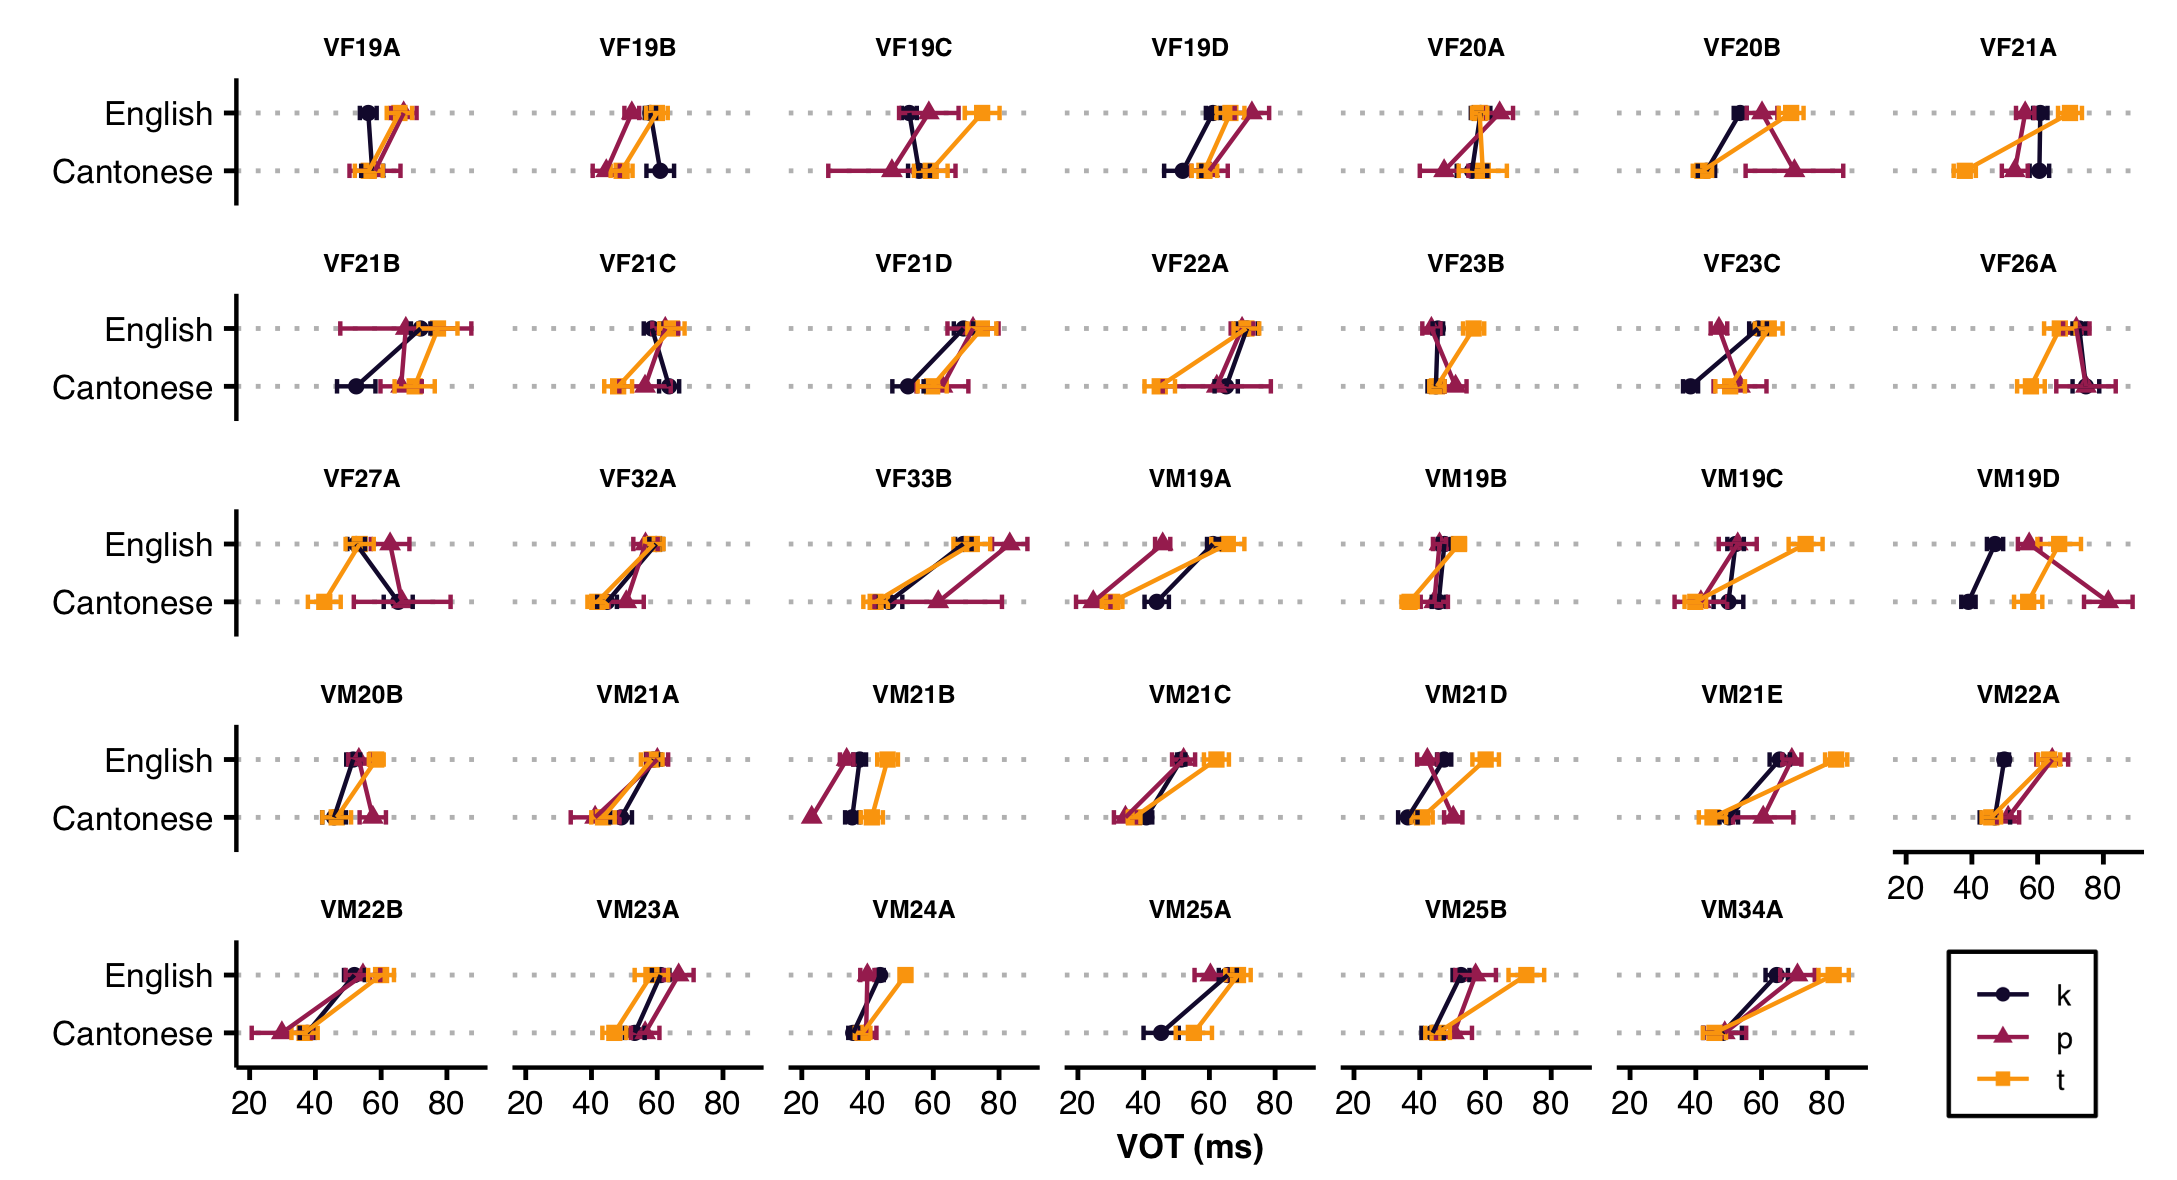
\includegraphics[width=\linewidth]{figures/4-ptk_vot_individuals.png}
  \caption{Mean and SE for VOT across place of articulation, language, and individuals in the SpiCE corpus.}
  \label{fig:ids}
\end{figure*}

Of the initial sample, 29.9\% was excluded, resulting in 9,458 long-lag stops, with Cantonese /\textipa{p}/: $n=374$, /\textipa{t}/: $n=1376$, and /\textipa{k}/ $n=1687$; and English /\textipa{p}/ $n=1129$, /\textipa{t}/ $n=1497$, and /\textipa{k}/ $n=3395$. Talkers had a median of 97 Cantonese stops (range: 59-194) and 166 English stops (range: 69-574). The higher number of English stops is likely due to lexical distributional reasons. The SpiCE corpus has a similar amount of recorded speech in each language, and while Cantonese stops were culled at a slightly higher rate in the exclusions specified above, they made up a smaller proportion to begin with (33\% of initial sample vs. 29\% of sample before excluding ``to''). English also seems to have more highly frequent /\textipa{k}/-initial word types. Conversely, Cantonese /\textipa{p}/ occurs in fewer, less frequent word types in the final sample ($n=60$, max frequency of 97) than English ($n=185$, max frequency of 214).

\section{Analysis \& Results}
The articulatory uniformity framework offers strong theoretical grounds for interpreting the structure of VOT variation within and across talkers. The analysis qualifies and quantifies that structure from a few different perspectives. In all cases, the pattern of results is depicted by Figure \ref{fig:ids}, which plots individuals' mean and standard errors for each of the three stops by language---showcasing both variability and commonalities.

\subsection{Ordinal relationships}
Prior work with lab and read speech strongly suggests an expected ordinal relationship for VOT across places of articulation: /\textipa{p}/ $<$ /\textipa{t}/ $<$ /\textipa{k}/. One of the major contributions of \citep{chodroff_2017_structure} is that these relationships are tighter that would be expected from a purely ordinal perspective. While ordinal relationships are a starting place, they represent just one piece of the puzzle. 

The results for the SpiCE corpus suggest that \textit{puzzle} is an appropriate characterization, as talkers largely did not adhere the expected order. Table \ref{tab:ordrel} reports the proportion of talkers whose mean VOT values followed the expected /\textipa{p}/ $<$ /\textipa{t}/ $<$ /\textipa{k}/ relationships. Prior work on connected speech reports rates of adherence in the 80-90\% range \citep{chodroff_2019_l2}, with the exception of English /\textipa{t}/ $<$ /\textipa{k}/ being drastically lower for native English speakers. While the /\textipa{t}/ $<$ /\textipa{k}/ comparison is also low here (18\%), only the English /\textipa{p}/ $<$ /\textipa{t}/ proportion (0.74) is at all close to previous work. This lack of adherence is apparent in the relative ordering or markers in Figure \ref{fig:ids}, though in many cases the standard errors overlap, suggesting that a strict ordering by means may not be appropriate. Additionally, crossed lines in Figure \ref{fig:ids} indicated that many talkers are not internally consistent across languages. 

\begin{table}[th]
\caption{Proportion of talker means that adhered to expected ordinal relationship for VOT: /p/ $<$ /t/ $<$/ k/ VOT durations. Note that talker VM25A has no instances of Cantonese /\textipa{p}/ in the sample.}
  \label{tab:ordrel}
  \centering
  \begin{tabular}{lllll}
    \toprule
    \textbf{Language} & \textbf{\textipa{p$<$t}} & \textbf{\textipa{t$<$k}} & \textbf{\textipa{p$<$k}} & n \\
    \midrule
    Cantonese	& 0.27	& 0.61	& 0.40	& 33 \\
    English	    & 0.74	& 0.18	& 0.41	& 34 \\
    \bottomrule
  \end{tabular}
\end{table}

\subsection{Pairwise correlations}

To examine the relationship between stops within and across languages, 15 pairwise Pearson's \textit{r} correlations were calculated across talker means and are reported along with Holm-adjusted p-values where significant. In each case, means were calculated over \textit{residual} VOT values from a simple linear regression in which VOT was predicted by average phone duration within the word---a proxy for speech rate calculated as the the difference between the AutoVOT-estimated onset and the force-aligned word offset, divided by the number of segments in the canonical form of the word. Using residual VOT means mitigates the impact of talker- and language-specific speech rate for these comparisons. This is important, as speech rate is known to influence VOT \citep{chodroff_2017_structure}, and because prior work demonstrate talker and language effects on speech rate \citep{bradlow_2017_rate}. 

Table \ref{tab:correlations} summarizes the output of the significant correlations. While there is some evidence for both within- and across-language structured variation, the correlations reported here are considerably lower compared to prior work on English connected speech, where similar within-language comparisons had $r>0.7$ \citep{chodroff_2017_structure,chodroff_2019_l2}. With the exception of the English /\textipa{p}/ $\sim$ /\textipa{k}/ ($r=0.75$, $p<0.001$), all of the correlations were either moderate ($0.5<r<0.7$; $p<0.01$) or not significant. Within-language correlations more consistently occurred (5 of 6 significant), compared to the across-language comparisons (3 of 9). Notably, most of the comparisons involving /\textipa{t}/ in either language, were not significant. While these relationships seem to indicate some degree of articulatory reuse, the overall picture is not particularly compelling. 

\begin{table}[hbt]
\caption{Correlations based on mean residual VOT by talker and language. Each row indicates the comparison, Pearson's \textit{r}, and Holm-adjusted p-value.}
  \label{tab:correlations}
  \centering
  \begin{tabular}{lll}
    \toprule
\textbf{Comparison}			& \textbf{\textit{r}}	& \textbf{\textit{p}} \\
\midrule
Cantonese /\textipa{p}/ $\sim$ Cantonese /\textipa{t}/   &	0.59	&	0.004 \\
Cantonese /\textipa{p}/ $\sim$ Cantonese /\textipa{k}/   &	0.54	&	0.009 \\
Cantonese /\textipa{t}/ $\sim$ Cantonese /\textipa{k}/   &	0.33	&	0.28 \\
English /\textipa{p}/ $\sim$ English /\textipa{t}/	     &	0.58	&	0.004 \\
English /\textipa{p}/ $\sim$ English /\textipa{k}/	     &	0.75 	&	$<$0.001 \\
English /\textipa{t}/ $\sim$ English /\textipa{k}/	     &	0.57	&	0.005 \\
Cantonese /\textipa{p}/ $\sim$ English /\textipa{p}/	 &	0.57	&	0.006 \\
Cantonese /\textipa{t}/ $\sim$ English /\textipa{t}/	 &	0.31	&	0.29 \\
Cantonese /\textipa{k}/ $\sim$ English /\textipa{k}/	 &	0.55	&	0.006 \\
Cantonese /\textipa{p}/ $\sim$ English /\textipa{t}/	 &	0.23	&	0.33 \\
Cantonese /\textipa{p}/ $\sim$ English /\textipa{k}/	 &	0.35	&	0.29 \\
Cantonese /\textipa{t}/ $\sim$ English /\textipa{p}/	 &	0.43	&	0.08 \\
Cantonese /\textipa{t}/ $\sim$ English /\textipa{k}/	 &	0.31	&	0.29 \\
Cantonese /\textipa{k}/ $\sim$ English /\textipa{p}/	 &	0.56	&	0.006 \\
Cantonese /\textipa{k}/ $\sim$ English /\textipa{t}/	 &	0.24	&	0.33 \\
    \bottomrule
  \end{tabular}
\end{table}

\subsection{Linear mixed effect model}
In an effort to better account for variation due to known factors such as speech rate and the presence of a preceding pause, a linear mixed effect model was fit with the \textit{lme4} R package \citep{bates_2015_lme4}. The aims of the model were two-fold: estimating the effect of language by segment, and elucidating the sources of variation in the random effect structure. The dependent variable, VOT (centered) was predicted by Average Phone Duration (standardized), Preceding Pause (False$=-0.32$, True$=1$), Language (Cantonese$=-1.75$, English$=1$), Place of Articulation (Place T: /\textipa{p}/$=-1.91$, /\textipa{t}/$=1$, /\textipa{k}/$=0$ ; Place K: /\textipa{p}/$=-3.38$, /\textipa{t}/$=10$, /\textipa{k}/$=1$), and the Language $\times$ Place interaction. As likely apparent from the parenthetical values, all categorical fixed effects were weighted effect coded \citep[following][]{chodroff_2017_structure}. Random intercepts for Talker and Word were included, as were by-Talker slopes for Language, Place, and their interaction.\footnote{Formula: VOT $\sim$ 1 $+$ Place $\times$ Language $+$ Average Phone Duration $+$ Preceding Pause $+$ (Place $\times$ Language $|$ Talker) $+$ (1 $|$ Word).}

The model returned a significant intercept ($\beta=3.62$, $SE=1.22$, $p=0.004$), significant main effects for Average Phone Duration ($\beta=7.75$, $SE=0.23$, $p<0.001$) and Preceding Pause (True; $\beta=2.96$, $SE=0.38$, $p<0.001$) as well as significant simple effect for Language (English; $\beta=2.81$, $SE=0.59$, $p<0.001$), indicating that VOT was longer at slower speech rates, as well as after pauses and in English, compared to the weighted mean. Neither Place nor its interaction with Language was significant. As one of the mixed effect model analysis goals was to assess the effect of Language across places of articulation, pairwise post-hoc comparisons were computed for Language by Place of Articulation using emmeans, with a confidence level of 0.95, and the Kenward-Roger degrees-of-freedom method. The contrast between languages was significant for /\textipa{t}/ ($\beta=-7.96$, $SE=2.25$, $p<0.001$) and /\textipa{k}/ ($\beta=-9.66$, $SE=2.43$, $p<0.001$), but not for /\textipa{p}/ ($\beta=-0.81$, $SE=2.28$, $p=0.78$). This suggests that VOT is consistently longer in English for /\textipa{t}/ and /\textipa{k}/.

The second goal of the mixed effects analysis was to gain insight into the sources of variation through the random effects structure. Of the random effects, the intercepts for Word ($SD=11.45$) and Talker ($SD=6.11$) accounted for the most variation, followed by the by-Talker slope standard deviations for Language ($SD=1.76$), Place T ($SD=2.76$), Place T $\times$ Language ($SD=1.53$), Place K ($SD=1.80$) and Place K $\times$ Language ($SD=1.03$). This indicates that talkers and words differ substantially in mean VOT, and that the slopes for Place and Language effects are more consistent across talkers.

\section{Discussion}

This paper reports a study of long-lag stops in Cantonese-English bilingual speech from the SpiCE corpus \citep{johnson_2020_spice}, and uses the uniformity framework to assess VOT similarity within and across languages. In broad strokes, the evidence for uniformity both within and across languages was limited. A correlation analysis provides evidence for within-language uniformity and some across-language structure. The magnitudes were mostly moderate, and most did not involve coronal stops. These results are corroborated by the random effects structure of the linear mixed effects model, as more of the variation is attributable to talker intercepts than to the Language and Place slope effects. In this sense, while there is some degree of structure in VOT variation, it seems to be weaker than the evidence in prior work, where strong within-language patterns were observed \citep{chodroff_2017_structure,chodroff_2019_l2}.

The far more interesting outcomes relate to unexpected results. The ordinal relationships should be interpreted with a grain of salt, as there are a number of potential explanations not immediately relevant to the research question. For example, means were based off of fewer tokens than in prior work (especially for /\textipa{p}/), which may render those proportions less reliable; and, the speech in SpiCE differs in style (conversational vs. read). Lastly, the error often overlaps, potentially making the ordinal relationships unreliable or less meaningful. Another unexpected outcome is that English VOT seems to be consistently longer than in Cantonese---the opposite of what prior work suggested \citep{clumeck_1981_cantonese,lisker_1964_vot}. No explanation is offered here other than to reiterate the casual speech style under examination, and that lab and corpus results often differ \citep{gahl_2012_reduce}, as do corpus studies of monolingual and bilingual speech \citep{johnson_2019_probabilistic}. 

While the results here do not necessarily provide evidence for a crosslinguistic uniformity constraint, they offer insight into what makes bilingual speech unique, as well as empirical descriptions of bilingual long-lag stop. In terms of describing the relationship between the long-lag stops in each language, talkers seem to maintain a crosslinguistic contrast despite the close proximity of the stops---for many talkers---in the long-lag space. This makes a composite category in SLM-r terms seem plausible \citep{flege_2021_slmr}, and merits further investigation. 

A lack of strong cross-language uniformity has implications for speech perception, in which tracking a uniformity-like constraint has been proposed as mechanism for rapidly adapting to speech across languages \citep{reinisch_2013_retune}, and in multilingual talker identification \citep{orena_2019_identifying}. If the results of this study persist, then such a constraint may have limited use in real communicative contexts, whether or not listeners use it in a lab setting. On the whole, this study highlights the need to study spontaneous speech, and offers a first pass at leveraging the methods of the uniformity framework to better understand crosslinguistic similarity.

\endinput % -------------------------------------------------------- %